\chapter{Echocardiography}
\label{ch:echocardiography}

% Chapter-opening illustrated modality infographic.
\begin{center}
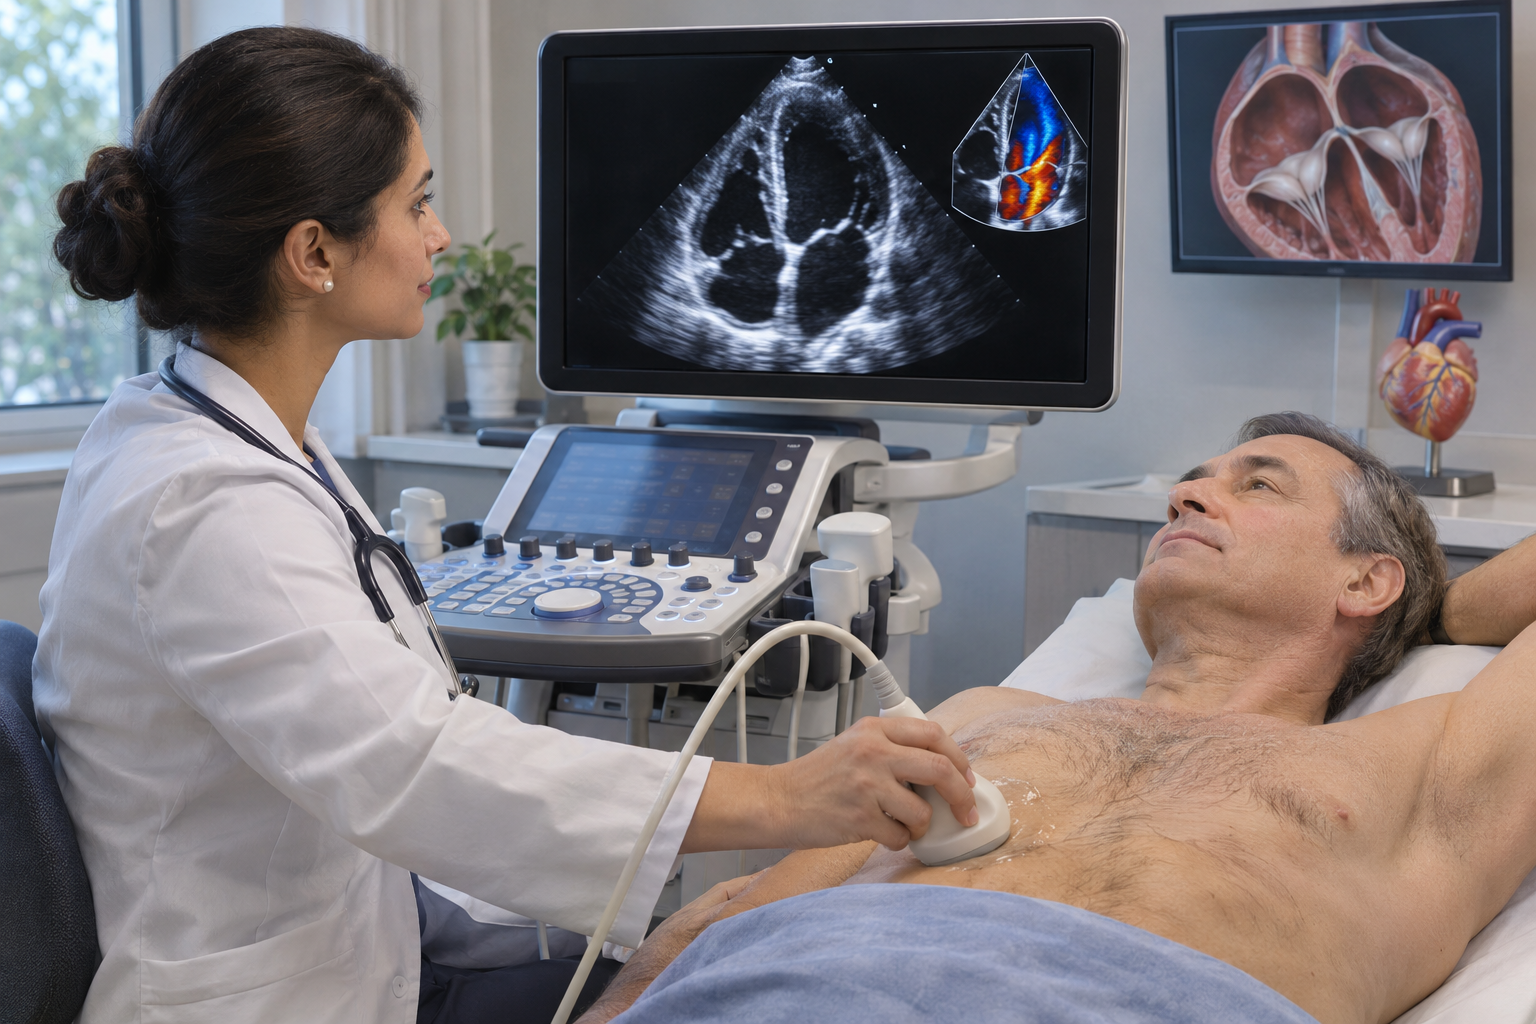
\includegraphics[width=\textwidth,keepaspectratio]{modalities/infographics/echocardiography_realistic.png}
\end{center}
\begin{center}\footnotesize Echocardiography uses ultrasound views and Doppler to assess cardiac structure, motion, and blood flow; measurements require clinical context. AI-generated illustration; echo panels are not clinical studies.\end{center}

\section{Overview}
Echocardiography is a specialized ultrasound imaging technique that evaluates cardiac anatomy, myocardial function, valvular function, intracardiac blood flow, and hemodynamics. It is one of the principal diagnostic imaging modalities used in cardiology.

This catalogue focuses on diseases and conditions for which echocardiography has established clinical utility. It includes transthoracic echocardiography (TTE), transesophageal echocardiography (TEE), stress echocardiography, Doppler echocardiography, and three-dimensional echocardiography.

\section{Where echocardiography is used}
The following numbered entries present common diagnostic applications by disease category. Findings should be interpreted with clinical information, appropriate views, and quantitative measurements.

\subsection{Cardiomyopathies}
\begin{enumerate}[leftmargin=*,itemsep=0.45em,topsep=0.4em]
\item \textbf{Alcohol-induced cardiomyopathy.} Useful imaging findings include: Ventricular dilatation and systolic dysfunction.
\item \textbf{Arrhythmogenic right ventricular cardiomyopathy.} Useful imaging findings include: Right ventricular dilatation and regional dysfunction.
\item \textbf{Cardiac amyloidosis.} Useful imaging findings include: Increased wall thickness and relative apical strain sparing may raise suspicion but are not diagnostic or subtype-specific.
\item \textbf{Cardiac sarcoidosis.} Useful imaging findings include: Regional dysfunction, basal septal thinning.
\item \textbf{Chemotherapy-induced cardiomyopathy.} Useful imaging findings include: Reduced ejection fraction or global longitudinal strain.
\item \textbf{Dilated cardiomyopathy.} Useful imaging findings include: Ventricular dilatation, reduced systolic function.
\item \textbf{Endomyocardial fibrosis.} Useful imaging findings include: Apical obliteration and restrictive filling.
\item \textbf{Hypertensive heart disease.} Useful imaging findings include: Left ventricular hypertrophy, diastolic dysfunction.
\item \textbf{Hypertrophic cardiomyopathy.} Useful imaging findings include: Abnormal myocardial hypertrophy.
\item \textbf{Hypertrophic obstructive cardiomyopathy.} Useful imaging findings include: Left ventricular outflow tract obstruction.
\item \textbf{Ischemic cardiomyopathy.} Useful imaging findings include: Regional wall-motion abnormalities.
\item \textbf{Left ventricular noncompaction.} Useful imaging findings include: Prominent trabeculations; interpret with ventricular function and clinical context, since trabeculation alone is not diagnostic.
\item \textbf{Peripartum cardiomyopathy.} Useful imaging findings include: Reduced left ventricular systolic function.
\item \textbf{Restrictive cardiomyopathy.} Useful imaging findings include: Restrictive ventricular filling pattern.
\item \textbf{Takotsubo cardiomyopathy.} Useful imaging findings include: Transient regional ventricular ballooning.
\end{enumerate}

\subsection{Valvular heart diseases}
\begin{enumerate}[leftmargin=*,itemsep=0.45em,topsep=0.4em]
\item \textbf{Aortic regurgitation.} Useful imaging findings include: Retrograde diastolic flow.
\item \textbf{Aortic stenosis.} Useful imaging findings include: Restricted leaflet opening, elevated pressure gradient.
\item \textbf{Bicuspid aortic valve.} Useful imaging findings include: Two functional aortic valve cusps.
\item \textbf{Carcinoid heart disease.} Useful imaging findings include: Thickened, retracted right-sided valve leaflets.
\item \textbf{Chordae tendineae rupture.} Useful imaging findings include: Disrupted chordal support with leaflet flail.
\item \textbf{Flail mitral leaflet.} Useful imaging findings include: Abnormal leaflet motion into the left atrium.
\item \textbf{Mitral annular calcification.} Useful imaging findings include: Echogenic calcification of the mitral annulus.
\item \textbf{Mitral regurgitation.} Useful imaging findings include: Retrograde systolic flow.
\item \textbf{Mitral stenosis.} Useful imaging findings include: Restricted leaflet opening, reduced valve area.
\item \textbf{Mitral valve prolapse.} Useful imaging findings include: Systolic displacement of mitral leaflets.
\item \textbf{Papillary muscle rupture.} Useful imaging findings include: Papillary muscle disruption, severe mitral regurgitation.
\item \textbf{Paravalvular leakage.} Useful imaging findings include: Regurgitant flow surrounding the prosthetic valve.
\item \textbf{Prosthetic valve regurgitation.} Useful imaging findings include: Abnormal regurgitant flow.
\item \textbf{Prosthetic valve stenosis.} Useful imaging findings include: Elevated transprosthetic pressure gradient; interpret with flow, valve type and size, and other Doppler measures.
\item \textbf{Prosthetic valve thrombosis.} Useful imaging findings include: Restricted prosthetic leaflet motion.
\item \textbf{Pulmonary valve regurgitation.} Useful imaging findings include: Retrograde diastolic flow.
\item \textbf{Pulmonary valve stenosis.} Useful imaging findings include: Elevated transpulmonary flow velocity.
\item \textbf{Rheumatic heart disease.} Useful imaging findings include: Leaflet thickening, commissural fusion.
\item \textbf{Tricuspid regurgitation.} Useful imaging findings include: Retrograde systolic flow.
\item \textbf{Tricuspid stenosis.} Useful imaging findings include: Restricted valve opening, increased pressure gradient.
\end{enumerate}

\subsection{Heart failure and ventricular dysfunction}
\begin{enumerate}[leftmargin=*,itemsep=0.45em,topsep=0.4em]
\item \textbf{Biventricular dysfunction.} Useful imaging findings include: Impaired function of both ventricles.
\item \textbf{Heart failure with mildly reduced ejection fraction (HFmrEF).} Useful imaging findings include: Mildly reduced ejection fraction.
\item \textbf{Heart failure with preserved ejection fraction (HFpEF).} Useful imaging findings include: Preserved ejection fraction; diastolic measures can support but do not establish the diagnosis without clinical context.
\item \textbf{Heart failure with reduced ejection fraction (HFrEF).} Useful imaging findings include: Reduced left ventricular ejection fraction.
\item \textbf{Left atrial enlargement.} Useful imaging findings include: Increased left atrial volume.
\item \textbf{Left ventricular diastolic dysfunction.} Useful imaging findings include: Abnormal ventricular relaxation and filling.
\item \textbf{Left ventricular dilatation.} Useful imaging findings include: Increased ventricular chamber dimensions.
\item \textbf{Left ventricular hypertrophy.} Useful imaging findings include: Increased myocardial wall thickness or mass.
\item \textbf{Right atrial enlargement.} Useful imaging findings include: Increased right atrial dimensions.
\item \textbf{Right ventricular dilatation.} Useful imaging findings include: Enlarged right ventricular chamber.
\item \textbf{Right ventricular failure.} Useful imaging findings include: Reduced right ventricular systolic function.
\item \textbf{Right ventricular hypertrophy.} Useful imaging findings include: Increased right ventricular wall thickness.
\end{enumerate}

\subsection{Ischemic heart disease}
\begin{enumerate}[leftmargin=*,itemsep=0.45em,topsep=0.4em]
\item \textbf{Acute myocardial infarction.} Useful imaging findings include: Regional wall-motion abnormalities.
\item \textbf{Hibernating myocardium.} Useful imaging findings include: Dysfunctional myocardium with contractile reserve.
\item \textbf{Ischemic mitral regurgitation.} Useful imaging findings include: Leaflet tethering and regurgitant flow.
\item \textbf{Left ventricular aneurysm.} Useful imaging findings include: Dyskinetic ventricular outpouching.
\item \textbf{Left ventricular free-wall rupture.} Useful imaging findings include: Myocardial disruption, hemopericardium.
\item \textbf{Left ventricular pseudoaneurysm.} Useful imaging findings include: Contained ventricular rupture.
\item \textbf{Myocardial ischemia.} Useful imaging findings include: Inducible wall-motion abnormalities during stress.
\item \textbf{Previous myocardial infarction.} Useful imaging findings include: Regional myocardial thinning and akinesia.
\item \textbf{Stunned myocardium.} Useful imaging findings include: Transient myocardial contractile dysfunction.
\item \textbf{Ventricular septal rupture.} Useful imaging findings include: Acquired interventricular communication.
\end{enumerate}

\subsection{Pericardial diseases}
\begin{enumerate}[leftmargin=*,itemsep=0.45em,topsep=0.4em]
\item \textbf{Cardiac tamponade.} Useful imaging findings include: Right-sided chamber collapse and respiratory flow variation.
\item \textbf{Congenital absence of the pericardium.} Useful imaging findings include: Abnormal cardiac position and mobility.
\item \textbf{Constrictive pericarditis.} Useful imaging findings include: Septal bounce and ventricular interdependence.
\item \textbf{Effusive-constrictive pericarditis.} Useful imaging findings include: Pericardial fluid with constrictive physiology.
\item \textbf{Hemopericardium.} Useful imaging findings include: Pericardial fluid, sometimes with echogenic clot.
\item \textbf{Pericardial cyst.} Useful imaging findings include: Extracardiac cystic structure.
\item \textbf{Pericardial effusion.} Useful imaging findings include: Echo-free space surrounding the heart.
\end{enumerate}

\subsection{Congenital heart diseases}
\begin{enumerate}[leftmargin=*,itemsep=0.45em,topsep=0.4em]
\item \textbf{Anomalous left coronary artery from pulmonary artery (ALCAPA).} Useful imaging findings include: Abnormal coronary origin and flow.
\item \textbf{Aortic valve atresia.} Useful imaging findings include: Absent direct flow through the aortic valve.
\item \textbf{Atrial septal defect (ASD).} Useful imaging findings include: Interatrial communication.
\item \textbf{Atrioventricular septal defect.} Useful imaging findings include: Abnormal atrioventricular junction and septal defects.
\item \textbf{Coarctation of the aorta.} Useful imaging findings include: Aortic narrowing with accelerated blood flow.
\item \textbf{Congenital coronary artery fistula.} Useful imaging findings include: Abnormal coronary vascular communication.
\item \textbf{Congenital corrected transposition.} Useful imaging findings include: Atrioventricular and ventriculoarterial discordance.
\item \textbf{Congenital submitral aneurysm.} Useful imaging findings include: Ventricular outpouching beneath the mitral annulus.
\item \textbf{Cor triatriatum.} Useful imaging findings include: Abnormal membrane dividing an atrial chamber.
\item \textbf{Double-outlet right ventricle.} Useful imaging findings include: Both great arteries arising predominantly from the right ventricle.
\item \textbf{Ebstein anomaly.} Useful imaging findings include: Apical displacement of tricuspid valve leaflets.
\item \textbf{Hypoplastic left heart syndrome.} Useful imaging findings include: Underdeveloped left-sided cardiac structures.
\item \textbf{Interrupted aortic arch.} Useful imaging findings include: Discontinuity of the aortic arch.
\item \textbf{Partial anomalous pulmonary venous return.} Useful imaging findings include: Partial abnormal pulmonary venous drainage.
\item \textbf{Patent ductus arteriosus (PDA).} Useful imaging findings include: Persistent communication between aorta and pulmonary artery.
\item \textbf{Patent foramen ovale (PFO).} Useful imaging findings include: Interatrial shunting, often demonstrated with bubble study.
\item \textbf{Persistent left superior vena cava.} Useful imaging findings include: Dilated coronary sinus, abnormal venous drainage.
\item \textbf{Pulmonary atresia.} Useful imaging findings include: Absent direct flow through the pulmonary valve.
\item \textbf{Sinus of Valsalva aneurysm.} Useful imaging findings include: Abnormal aortic sinus dilatation.
\item \textbf{Tetralogy of Fallot.} Useful imaging findings include: VSD, overriding aorta, right ventricular outflow obstruction and hypertrophy.
\item \textbf{Total anomalous pulmonary venous return.} Useful imaging findings include: Abnormal pulmonary venous drainage.
\item \textbf{Transposition of the great arteries.} Useful imaging findings include: Ventriculoarterial discordance.
\item \textbf{Tricuspid atresia.} Useful imaging findings include: Absent functional tricuspid valve opening.
\item \textbf{Truncus arteriosus.} Useful imaging findings include: Single common arterial trunk.
\item \textbf{Ventricular septal defect (VSD).} Useful imaging findings include: Interventricular communication.
\end{enumerate}

\subsection{Cardiac infections and inflammatory diseases}
\begin{enumerate}[leftmargin=*,itemsep=0.45em,topsep=0.4em]
\item \textbf{Cardiac fistula associated with endocarditis.} Useful imaging findings include: Abnormal intracardiac flow communication.
\item \textbf{Infective endocarditis.} Useful imaging findings include: Possible vegetations or complications; a negative TTE does not exclude disease when clinical suspicion remains.
\item \textbf{Libman--Sacks endocarditis.} Useful imaging findings include: Sterile valvular vegetations.
\item \textbf{Myocarditis.} Useful imaging findings include: Global or regional ventricular dysfunction.
\item \textbf{Nonbacterial thrombotic endocarditis.} Useful imaging findings include: Sterile valvular masses.
\item \textbf{Perivalvular abscess.} Useful imaging findings include: Abnormal perivalvular cavity or thickening.
\item \textbf{Prosthetic valve endocarditis.} Useful imaging findings include: Possible vegetation, prosthetic dysfunction or dehiscence; prosthetic shadowing can limit TTE and TEE.
\item \textbf{Rheumatic carditis.} Useful imaging findings include: Valvular inflammation and regurgitation.
\end{enumerate}

\subsection{Intracardiac tumors and masses}
\begin{enumerate}[leftmargin=*,itemsep=0.45em,topsep=0.4em]
\item \textbf{Atrial myxoma.} Useful imaging findings include: Mobile intracavitary mass.
\item \textbf{Cardiac angiosarcoma.} Useful imaging findings include: Irregular infiltrative mass.
\item \textbf{Cardiac fibroma.} Useful imaging findings include: Solid intramyocardial mass.
\item \textbf{Cardiac lipoma.} Useful imaging findings include: Well-defined cardiac mass.
\item \textbf{Cardiac lymphoma.} Useful imaging findings include: Infiltrative myocardial or intracardiac mass.
\item \textbf{Cardiac metastases.} Useful imaging findings include: Abnormal myocardial or pericardial masses.
\item \textbf{Cardiac papillary fibroelastoma.} Useful imaging findings include: Small mobile valvular mass.
\item \textbf{Cardiac rhabdomyoma.} Useful imaging findings include: Intramyocardial masses.
\item \textbf{Lambl excrescences.} Useful imaging findings include: Thin filamentous valvular structures.
\item \textbf{Left atrial appendage thrombus.} Useful imaging findings include: Intracavitary mass visualized predominantly with TEE.
\item \textbf{Left atrial thrombus.} Useful imaging findings include: Mass within the left atrium.
\item \textbf{Left ventricular thrombus.} Useful imaging findings include: Intracavitary mass, frequently near the apex.
\item \textbf{Right atrial thrombus.} Useful imaging findings include: Intracavitary right atrial mass.
\item \textbf{Right ventricular thrombus.} Useful imaging findings include: Intracavitary right ventricular mass.
\end{enumerate}

\subsection{Aortic diseases}
\begin{enumerate}[leftmargin=*,itemsep=0.45em,topsep=0.4em]
\item \textbf{Aortic annuloectasia.} Useful imaging findings include: Dilatation of the aortic annulus and root.
\item \textbf{Aortic atherosclerosis.} Useful imaging findings include: Echogenic aortic plaques.
\item \textbf{Aortic dissection.} Useful imaging findings include: Intimal flap may be seen in accessible segments; echocardiography does not assess the entire aorta.
\item \textbf{Aortic intramural hematoma.} Useful imaging findings include: Possible aortic wall thickening; findings are nonspecific and CT or MRI is generally needed.
\item \textbf{Aortic root abscess.} Useful imaging findings include: Abnormal periannular cavity.
\item \textbf{Aortic root dilatation.} Useful imaging findings include: Increased aortic root diameter.
\item \textbf{Ascending aortic aneurysm.} Useful imaging findings include: Enlarged ascending aorta.
\end{enumerate}

\subsection{Pulmonary circulation}
\begin{enumerate}[leftmargin=*,itemsep=0.45em,topsep=0.4em]
\item \textbf{Acute pulmonary embolism.} Useful imaging findings include: Possible right ventricular strain or dilatation; a normal echocardiogram does not exclude PE.
\item \textbf{Chronic thromboembolic pulmonary hypertension.} Useful imaging findings include: Right ventricular hypertrophy and pressure overload; echocardiography does not identify the thromboembolic obstruction.
\item \textbf{Cor pulmonale.} Useful imaging findings include: Right ventricular structural and functional abnormalities.
\item \textbf{Eisenmenger syndrome.} Useful imaging findings include: Pulmonary hypertension with bidirectional or reversed shunting.
\item \textbf{Pulmonary artery aneurysm.} Useful imaging findings include: Pulmonary artery dilatation.
\item \textbf{Pulmonary artery stenosis.} Useful imaging findings include: Localized flow acceleration.
\item \textbf{Pulmonary hypertension.} Useful imaging findings include: Elevated estimated pulmonary pressure; echocardiography estimates probability and does not replace catheter confirmation when indicated.
\end{enumerate}

Echocardiography can demonstrate the hemodynamic consequences of pulmonary embolism but cannot reliably exclude it.

When endocarditis remains clinically suspected despite a nondiagnostic study, additional imaging, often TEE, may be required. The choice depends on the patient, suspected complication, and initial image quality.

\subsection{Postoperative and device-related conditions}
\begin{enumerate}[leftmargin=*,itemsep=0.45em,topsep=0.4em]
\item \textbf{Cardiac device-related perforation.} Useful imaging findings include: Abnormal lead position, possible pericardial effusion.
\item \textbf{Left atrial appendage occluder leakage.} Useful imaging findings include: Residual flow around the occlusion device.
\item \textbf{Left ventricular assist device obstruction.} Useful imaging findings include: Abnormal cannula flow characteristics.
\item \textbf{Pacemaker lead-associated endocarditis.} Useful imaging findings include: Vegetation attached to intracardiac lead.
\item \textbf{Pacemaker lead-associated thrombus.} Useful imaging findings include: Mass attached to intracardiac lead.
\item \textbf{Prosthetic valve dehiscence.} Useful imaging findings include: Abnormal rocking motion of prosthetic valve.
\item \textbf{Residual atrial septal defect.} Useful imaging findings include: Persistent interatrial shunting.
\item \textbf{Residual ventricular septal defect.} Useful imaging findings include: Persistent interventricular shunting.
\end{enumerate}

\subsection{Summary}
\begin{center}
\begin{tabular}{@{}p{0.70\textwidth}r@{}}
\toprule
\textbf{Disease category} & \textbf{Entries} \\
\midrule
Aortic diseases & 7 \\
Cardiomyopathies & 15 \\
Congenital heart diseases & 25 \\
Heart failure and ventricular dysfunction & 12 \\
Infections and inflammatory diseases & 8 \\
Intracardiac tumors and masses & 14 \\
Ischemic heart disease & 10 \\
Pericardial diseases & 7 \\
Postoperative and device-related conditions & 8 \\
Pulmonary circulation & 7 \\
Valvular heart diseases & 20 \\
\midrule
\textbf{Total} & \textbf{133} \\
\bottomrule
\end{tabular}
\end{center}

\subsection{Types of echocardiography}
\begin{longtable}{@{}p{0.40\textwidth}p{0.54\textwidth}@{}}
\toprule
\textbf{Technique} & \textbf{Primary diagnostic application} \\
\midrule
\endfirsthead
\toprule
\textbf{Technique} & \textbf{Primary diagnostic application} \\
\midrule
\endhead
2D echocardiography & Structural cardiac abnormalities \\
3D echocardiography & Volumetric and complex anatomical assessment \\
Color Doppler echocardiography & Abnormal intracardiac blood flow \\
Contrast echocardiography & Chamber delineation and shunt assessment \\
Fetal echocardiography & Congenital cardiac abnormalities \\
M-mode echocardiography & Cardiac dimensions and tissue motion \\
Speckle-tracking echocardiography & Myocardial deformation and strain \\
Spectral Doppler echocardiography & Flow velocities and pressure gradients \\
Stress echocardiography & Inducible myocardial ischemia \\
Tissue Doppler imaging & Myocardial tissue velocities \\
Transesophageal echocardiography (TEE) & Detailed valvular and intracardiac examination \\
Transthoracic echocardiography (TTE) & Routine cardiac structural and functional assessment \\
\bottomrule
\end{longtable}

\subsection{Quantitative parameters}
For developing an echocardiographic medical imaging dataset, the following measurements are particularly important.

\begin{longtable}{@{}p{0.64\textwidth}p{0.30\textwidth}@{}}
\toprule
\textbf{Parameter} & \textbf{Abbreviation} \\
\midrule
\endfirsthead
\toprule
\textbf{Parameter} & \textbf{Abbreviation} \\
\midrule
\endhead
Aortic valve area & AVA \\
Cardiac index & CI \\
Cardiac output & CO \\
Early-to-late transmitral flow velocity ratio & E/A \\
Effective regurgitant orifice area & EROA \\
Global longitudinal strain & GLS \\
Left atrial volume index & LAVI \\
Left ventricular ejection fraction & LVEF \\
Left ventricular end-diastolic volume & LVEDV \\
Left ventricular end-systolic volume & LVESV \\
Left ventricular mass index & LVMI \\
Mitral valve area & MVA \\
Pulmonary artery systolic pressure & PASP \\
Regurgitant fraction & RF \\
Regurgitant volume & RVol \\
Right ventricular fractional area change & RVFAC \\
Stroke volume & SV \\
Transmitral-to-annular early diastolic velocity ratio & E/e$^{\prime}$ \\
Tricuspid annular plane systolic excursion & TAPSE \\
\bottomrule
\end{longtable}

\subsection{Published medical images and datasets}
\begin{longtable}{@{}p{0.40\textwidth}p{0.54\textwidth}@{}}
\toprule
\textbf{Source} & \textbf{Primary utility} \\
\midrule
\endfirsthead
\toprule
\textbf{Source} & \textbf{Primary utility} \\
\midrule
\endhead
American Society of Echocardiography & Clinical guidelines and diagnostic criteria \\
CAMUS Dataset & Cardiac ultrasound segmentation \\
EchoNet-Dynamic & Annotated echocardiographic videos \\
Echopedia & Educational echocardiographic images \\
European Association of Cardiovascular Imaging & Cardiovascular imaging standards \\
PubMed Central & Published clinical images and videos \\
Radiopaedia & Clinical imaging cases \\
\bottomrule
\end{longtable}

\subsection{Selected clinical guidance}
The following professional guidance supports interpretation of the findings and limitations summarized in this chapter:
\begin{itemize}
\item \href{https://academic.oup.com/eurheartj/article/44/37/3503/7246608}{2023 ESC Guidelines for the management of cardiomyopathies} (trabeculation and cardiomyopathy assessment).
\item \href{https://ashpublications.org/bloodadvances/article/doi/10.1182/bloodadvances.2025017073/566264}{ASH clinical practice guidance on diagnosis of light-chain amyloidosis} (cardiac findings require etiologic confirmation).
\item \href{https://academic.oup.com/eurheartj/article/44/39/3948/7243107}{2023 ESC Guidelines for the management of endocarditis} (multimodality imaging and prosthetic-valve limitations).
\item \href{https://www.asecho.org/wp-content/uploads/2025/07/Left-Ventricular-Diastolic-Function.pdf}{ASE 2025 recommendations for evaluation of left ventricular diastolic function}.
\item \href{https://www.asecho.org/wp-content/uploads/2024/01/PIIS0894731723005333.pdf}{ASE guideline for evaluation of prosthetic valve function}.
\item \href{https://academic.oup.com/eurheartj/article/41/4/543/5556136}{2019 ESC Guidelines for acute pulmonary embolism} (echocardiography in risk assessment, not exclusion).
\end{itemize}

For medical imaging research, echocardiography should primarily be treated as a spatiotemporal imaging modality rather than a static image modality. Many abnormalities require an entire cardiac cycle, multiple anatomical views, and quantitative Doppler measurements.

